\documentclass[twoside=false,DIV=14]{scrartcl}
\input{./latex_setup.tex}
\usepackage{caption}
\captionsetup{labelformat=empty}

\title{\color{redish} \vspace{-1em}COMP3000: EPIC Programming Languages}

\begin{document}
{\color{blackish}\maketitle}\vspace{-7em}

\begin{abstract}
\end{abstract}
    Programming Languages is a third-year computing unit which combines \emph{computer science} and \emph{software engineering} and occupies a critical place in the Software Engineering and Software Technology programs of study.  In 2025 it was taught in an EPIC style which, while a natural fit for engineering units, is not so simply implemented for an applied mathematics like computer science.  


\begin{figure}[h]
    \begin{center}
      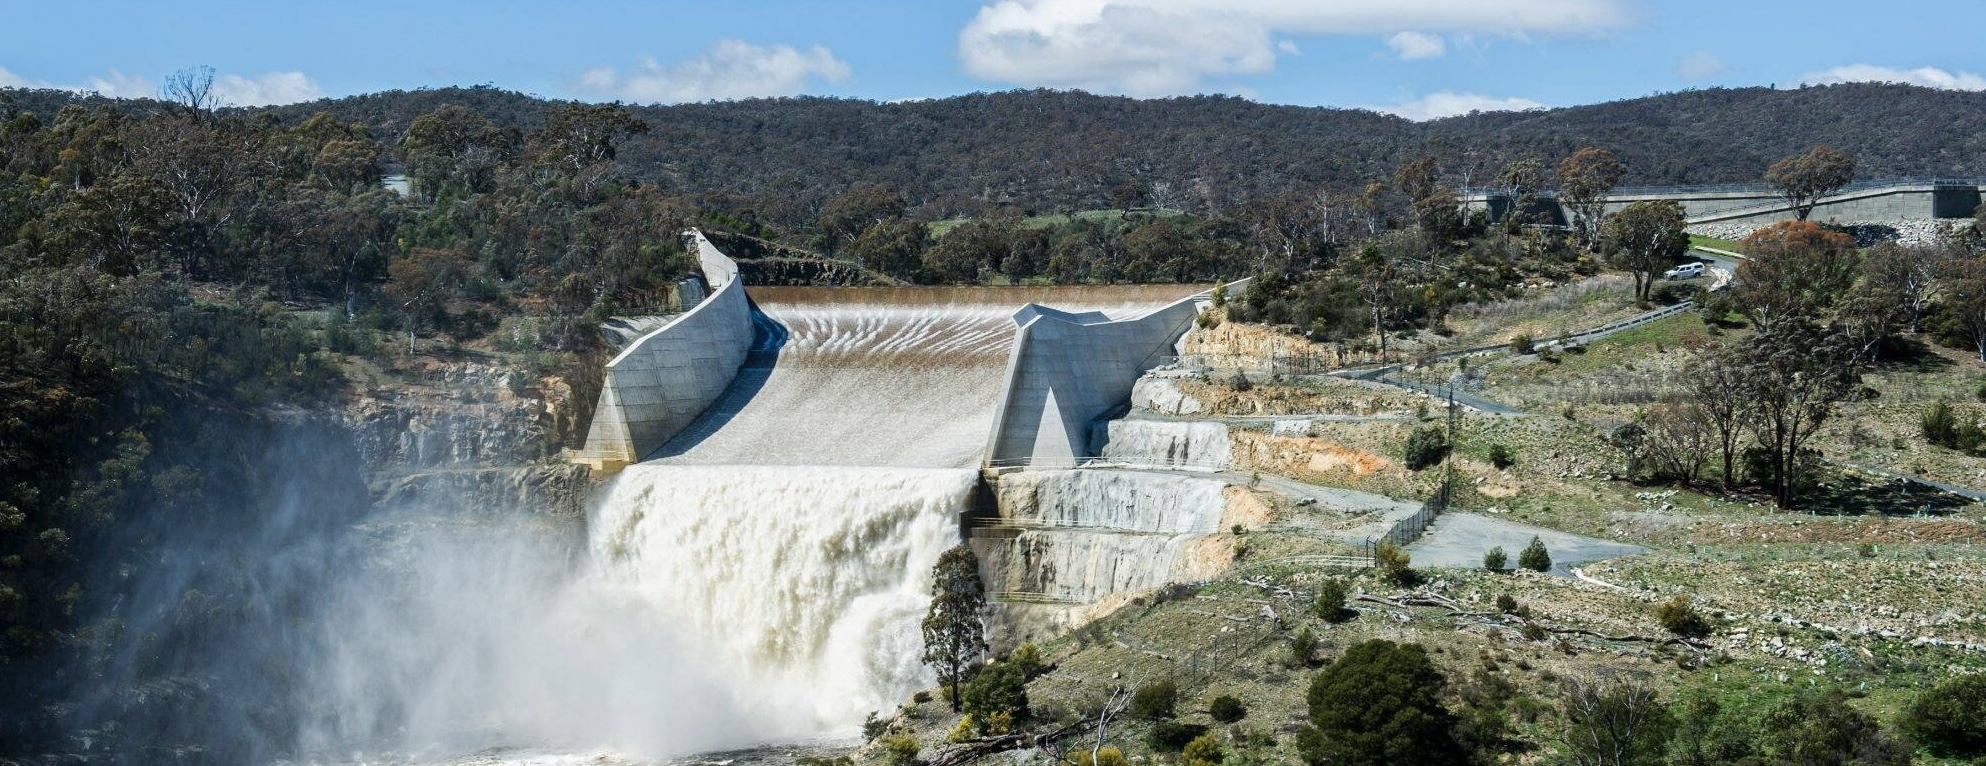
\includegraphics[width=0.8\textwidth]{googong.jpg}
    \end{center}
    \caption{The Googong Dam is one of the river flows students described.}
  \end{figure}
  
Modelling rivers involves taking rainfall data and simulating what water levels will result from that rainfall over a period of time.  This type of modelling is vital to environmental management and public safety. Floods can be predicted and mitigation methods can be designed.  It also allows water managers to experiment with different dam strategies to maximise safety.

River system modelling is normally done with simulation software but it could be done better if it was done with a \emph{custom programming language} instead.  COMP3000 students used what they learned to create just such a language.  Solving this problem is \emph{a real contribution to the science of waterflow management}.

\subsubsection*{Co-Design}
As students work through their workshops, unit staff adjusted future work to account for the directions students were taking and their choices.  In this way the course is \emph{co-designed} with each cohort of students.
  
This unit of study is also a \emph{content-heavy} unit with many complex concepts that need mastering to complete the learning outcomes.  In this document we describe this unit of study at a high level and show how content-heavy units can be an EPIC experience.

\begin{description}
\item[Experience that transforms] One of the career paths for students completing this unit is to join specialised software consultancies that help clients solve particularly difficult problems which normal consultancies have failed to solve and that is exactly what the students will experience in this unit of study.
\item[Purpose that inspires] The classwork will guide students through the task of creating a unique programming language with novel, real-world applications.  The students will see that the capability they are creating does not yet exist and will see how their work can fill that hole in the real world for a real client.  
\item[Impact that matters] In 2025 the classwork will revolve around creating a \emph{language} to model water flows in river systems.  While simulation-based approaches already exist, language-based solutions do not.  Language-based solutions require specific skills (those covered in this unit of study) which are not widely available but in return are more powerful, more flexible, more understandable, and more maintainable.  Each group will create their own such language and will demonstrate the value of it to interested parties.
\item[Collaboration that empowers] Classes are organised around \emph{Team Based Learning}.  Students work in teams on carefully calibrated activities which both re-inforce the fundamental concepts/skills \emph{and} allows them to creatively apply them as they choose.  There will be thirteen 2-hour collaborative classes accross semester at convenient times for students to choose from.  Students will form groups in the first week and work in those groups throughout all thirteen classes.
\end{description}

\begin{figure}[h]
    \begin{center}
    
\includegraphics[width=0.8\textwidth]{tbl.jpg}
\end{center}
\caption{Students will work collaboratively in all classes, acting as a specialist consultancy}
\end{figure}

\begin{tabular}{lcl}
\textbf{class \#} & \textbf{content and skills} & \textbf{EPIC activities} \\
\hline
1 & team based learning  & creating effective teams\\
2 & little languages & regular expression upskill \\
3 & lox & generating code for a graphics language from lox \\
4 & scanning & water flow modelling with programming languages \\
5 & abstract syntax trees and grammars & a simple language of water flows\\
6 & parsing grammars & parsing representations of water flows \\
7 & evaluation of expressions & computing water flows \\
8 & statements & exploration of student ideas \\
9 & statements & how variables lift expressiveness\\
10 & control flow & water flow management with dams \\
11 & functions & unlocking full power with functions \\
12 & functions & crafting a demonstration \\
13 & resolving & exploration of student ideas \\
\hline
\end{tabular}

\newpage

\section*{2025 Report}

A note for the reader.  The COMP3000 teaching team takes an approach to teaching which is \emph{not necessarily} a natural fit for certain approaches to EPIC.  In particular, we have never had good experiences with so-called "minimal instruction" approaches, nor been convinced by the research which attempts to support that approach.  We are constructivists who believe a teacher's job is a) to know the field so deeply and b) be experienced with students so that c) they can guide students from where they currently are on the right path for them to where they need to be.  We insist the teacher remains a lynchpin of the students learning experience even when moving to more student-led approaches or open-ended problems.  We note this because that approach colours our experience of EPIC and TBL and will surely come through in this review.  We hope those who don't share this view can still find value in our experience.

\begin{figure}
\begin{minipage}{0.4\textwidth}
\begin{tabular}{|l|l|l|}
  \hline
  week & tue 9am & tue 11 am \\ \hline
  2 & 26 & 29 \\
  3 & 19 & 22 \\
  4 & 22 & 23 \\
  5 & 19 & 21 \\
  6 & 18 & 18 \\
  7 & 14 & 20 \\
  8 & 12 & 19 \\
  9 & 15 & 21 \\
  10 & 11 & 17 \\
  11 & 12 & 19 \\
  12 & 6 & 13 \\
  13 & 3 & 9 \\
  \hline
\end{tabular}
\end{minipage}
\begin{minipage}{0.75\textwidth}
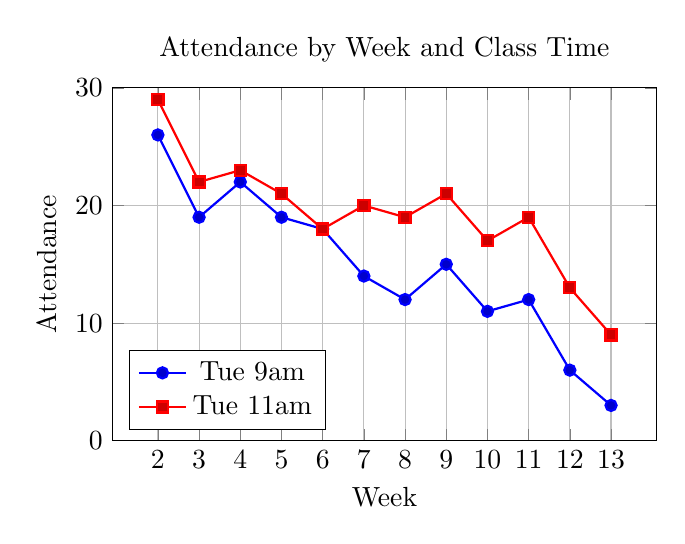
\begin{tikzpicture}
\begin{axis}[
    width=0.7\textwidth,
    height=0.5\textwidth,
    xlabel={Week},
    ylabel={Attendance},
    xtick={2,3,4,5,6,7,8,9,10,11,12,13},
    ymin=0, ymax=30,
    legend pos=south west,
    grid=major,
    title={Attendance by Week and Class Time}
]
\addplot+[mark=*, thick, color=blue] coordinates {
    (2,26) (3,19) (4,22) (5,19) (6,18) (7,14) (8,12) (9,15) (10,11) (11,12) (12,6) (13,3)
};
\addlegendentry{Tue 9am}

\addplot+[mark=square*, thick, color=red] coordinates {
    (2,29) (3,22) (4,23) (5,21) (6,18) (7,20) (8,19) (9,21) (10,17) (11,19) (12,13) (13,9)
};
\addlegendentry{Tue 11am}
\end{axis}
\end{tikzpicture}
\end{minipage}
\caption{Attendance trends for two classes of COMP3000 in 2025}
\label{fig:attendance}
\end{figure}
\begin{description}
\item[The classroom experience is more positive than usual] Despite how attendance diminished, the classroom was overrall a vibrant learning environment.  Class teachers are enjoying the experiece of TBL and we have had no negative feedback from students.
\item[Attendance is not high enough]  With the mandate against weekly grading, which was previously used in COMP3000 primarily to motivate attendance, we were concerned that attendance would drop.  We estimated we would end up around 30\% attendance but were seeing closer to 60\% attendance at the mid-semester break. Unfortunately, as can be seen in figure \ref{fig:attendance}, attendance dropped quickly after that.  Note that the two classes we monitored and which are shown in the plot were \emph{the most attended classes} meaning all other classes had less students attending.  We found application exercises stopped working being an effective use of time at around 15 students attending though we persisted to complete the semester.  Upon asking students how the classes were going, the most common response was "my team don't turn up but I am working well with the people who turn up".  We hope we can adjust in future by "pairing up" classes.  As attendance drops we will combine classes and merge teams so the second half of semester still benefits from the advantages of TBL.
\item[RATs are \emph{more} than preparation]  As we prepared for TBL we expected RATs would get students warmed-up and motivate them to do the pre-class preparation.  What we did not predict is the extent to which RATs would be a significant learning experience in their own right.  Students are learning from each other and from the class teachers during RATs and everyone seems to be enjoying the experience.  One result of this is that more time is being spent on RATs than we planned.
\item[RATs get the job done for exam preparation] We were concerned how students would perform in the exam given they had been doing open-ended application exercises for the bulk of the classes.  However, the engagement with RATs was very high and the final exam showed that students had succussfully prepared for this assessment.  We note that we did make the exam very RAT-like but feel confident we can relax that somewhat and students will still be prepared.
\item[The demands on class teachers are substantially greater than usual] Previously, class teachers would spend most of their time answering relatively easy questions about the content.  This semester the discussions went off on tangents and regularly hit subtle edge cases which required more skill and experience to handle well.  In one class I attended there was a discussion about what a global variable really means.  Only an experienced reader in programming languages can really answer that question.  The ability to do that discussion justice is beyond the ability of people who don't have a research masters or PhD in programming languages.  This is overall \emph{a good thing} since it means class is more engaging and more interesting, but it does need noting.  We see it as a tradeoff between precision and engagement (i.e. answers in class are not as precisely correct, but students are more engaged to hear it) and consider the tradeoff worth it.  Indeed we think that tradeoff is perhaps built into the spirit of EPIC.
\item[The teaching team needs more preparation time than usual] We have an extremely experienced and capable teaching team this semester and we are using 2 hours per teacher per week for preparation and could make good use of another hour per week.  At this point it looks like two hours per teacher per week is the minimum preparation time needed in EPIC3000.
\item[Directing students along a real world project is hard work]  The approach we have taken in EPIC3000 is to tackle a real-world problem within the context of the learning outcomes.  We sketched this out at the start of semester in a way we knew would work with some amount of work, but the devlish details are taking a lot of time and all our skill/experience to work through.  I've adopted the term "co-design" as we have had to constantly adjust each week's class content to account for the directions students are taking, their choices, and their misconceptions.  Getting ahead of the students and finding which parts of the domain will derail their learning is hard work and requires exploring all the possible paths students might take.  Then we need to communicate that to the full teaching team.  With experienced staff teaching the same course year-in and year-out this will get easier, but it seems likely we will need to change domains every couple of years which will reset the clock on that experience.  One way to protect against this is to ensure class teachers are doing 3 or more classes per week.
\item[Our worst worries have \emph{not} been realised]  Two concerns we had before begning were that a) attendance would quickly drop off and b) the highly interactive style would disadvantage introverted and neurodiverse students.  At the end of semester we can say that attendance did eventually drop off, but it seems to have held up better than other units.  We also found ourselves having lots of opportunities to support the neurodiverse students who attended class but can't account for any who did not.
\item[We can't keep doing application exercises during assessment season] As soon as the assignment specification was relesed, students wanted to work on that in class.  the RATs still ran but once students had the floor they were focussed on the upcomming assignment.  Combined with 3AM assessment season and the drop off in attendance, we have decided to stop trying to do normal application exercises in class and instead focus on the assignment during those two periods.  After the assignment was due, we crafted application exercises that encompass more than one week's work to start catching up.
\end{description}

\begin{figure}
\begin{minipage}{0.4\textwidth}
\begin{tabular}{|l|l|l|}
  \hline
  response & engaging & stressful \\ \hline
  much less & 5 & 4 \\
  a little less & 13 & 17 \\
  equally & 31 & 36 \\
  slightly more & 37 & 42 \\
  much more & 30 & 17 \\
  \hline
\end{tabular}
\end{minipage}
\begin{minipage}{0.75\textwidth}
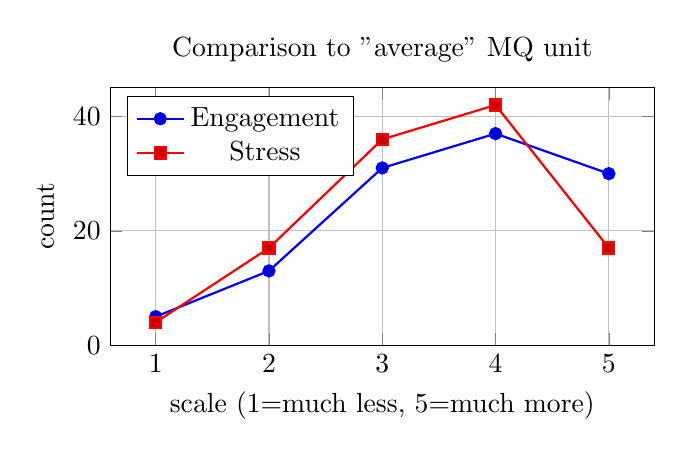
\begin{tikzpicture}
\begin{axis}[
    width=0.7\textwidth,
    height=0.4\textwidth,
    xlabel={scale (1=much less, 5=much more)},
    ylabel={count},
    xtick={0,1,2,3,4,5},
    ymin=0, ymax=45,
    legend pos=north west,
    grid=major,
    title={Comparison to "average" MQ unit}
]
\addplot+[mark=*, thick, color=blue] coordinates {
    (1,5) (2,13) (3,31) (4,37) (5,30)
};
\addlegendentry{Engagement}

\addplot+[mark=square*, thick, color=red] coordinates {
    (1,4) (2,17) (3,36) (4,42) (5,17)
};
\addlegendentry{Stress}
\end{axis}
\end{tikzpicture}
\end{minipage}
\caption{Student perspectives in week 8 of semester}
\label{fig:student_perspectives}
\end{figure}
The downsides we have observed which are related more to the EPIC aspects of the course are:
\begin{description}
\item[Real world domains are complex and hard to learn]  The domain of water flow modelling seemed like a simple one but it took a great deal of the student's cognitive load to work within it.  This extra cognitive load is an impediment to other learning.  It may still be a win overall, but the load is very substantial.  I would estimate 50\% of student cognitive load is going into learning the domain and only 50\% into learning the programming languages content.  One teacher remarked "I do find myself talking about evaporation and rainfall more than I imagined I would in this unit"
\item[Students head on the wrong path and need redirecting] This is not a surprise, but I think neglected sometimes when teaching units that reward exploration and creativity.  Giving students freedom to explore and a real-world problem to solve results in many teams going into dead ends early on.  Recovering from these dead ends is harder the longer they persist and takes skilled class teachers.  Teachers need to be much more than facilitators to support student in this situation.  Allowing them to continue pursuing the wrong path is robbing them of the chance to learn.
\item[Constant co-design is expensive and requires highly skilled staff]    We have found unit staff need to be constantly on the lookout for teams heading off in the wrong direction and need to intervene early and often to get them back on track.  The widely used term "co-design" is quite appropriate for what we have found ourselves doing in support of our students.  Getting the balance between freedom to explore and avoidance of dead ends is the main task class teachers have found themselves taking on during class time and the main use of senior staff time during semester.  We have tackled this by providing written and recorded guidance each week on the common approaches students are taking and the pitfalls they are encountering.  We are also publishing a "ground truth" solution each week which students can go to if their own approach is failing.   We worked hard to ensure the communication was two-way so that interesting student ideas got given airtime as well.  This was expensive in terms of staff time allocation.
\item[Making a submission from application exercises is key]  Class teachers report that students probably would not be engaging in the class exercises if they were not expecting to be assessed on them.  We have found a  way that matched 3AM and without it I think we would have lost too many students to vagrancy. 
\item[We can't ensure broad coverage of the material] Any real world domain will de-emphasise some aspect of the material and over-emphasise others.  We have done a good job finding a domain which covers most of the material well but the negative effect is still noticable. We would be very hesistant to recommend this approach in units which are pre-requisites for other units.
\item[Weak students are disadvantaged]  We've noticed that students who "don't get it" (i.e. just can't get going on a learning outcome for whatever reason), \emph{really don't get it in an EPIC setting}.  This makes sense because the inroads they might have had through graded scaffolded exercises is very much reduced in this setting.  We note these students can still generate the output they have been asked to (to a greater or lesser extent) but the lack of actualy understanding behind that generated output is noticably greater than last year. 
\end{description}

The upsides we have observed which are related more to the EPIC aspects of the course are:
\begin{description}
  \item[Students are more engaged than usual]  The domain problem is interesting in itself and giving students something to get into even if programming languages bores them.
  \item[Top students are thriving]  The best students are finding lots of interesting directions to explore and are enjoying the freedom to do so.  We note that the co-design aspect is key to supporting this.  Without such close interactions with unit staff on the matters of substance, these students would instead be frustrated that they have ideas their teammates don't share and that they can't explore them.
  \item[Unit staff are more engaged than usual]  The unit staff are also enjoying having a real-world problem to think through.  Again, the fact that each is effectively an extra team member to a number of teams via the co-design approach is key to this.  They get right into the "weeds" of the problem which is where all the fun is.
\end{description}

\subsubsection*{Student Perspectives}
We did a quick survey of students in week 8.  We asked students to rate on a scale of 1 (much less) to 5 (much more) how engaging and stressful this unit is compared to their "average" MQ unit.  The results are shown in figure \ref{fig:student_perspectives}.  Note that only students who attended class were involved.

Students find the unit both more engaging and more stressful.  The engagement increase is greater than the stress increase and our observations are that the stress is "productive" stress in most ways.  However, we think teachers planning to go down this path should be cognisant of the extra stress and be prepared to help students manage it.

The following is some unsolicited feeback we recieved from a student at the end of semester.
\begin{quote}
I just wanted to reach out to share my positive experience with COMP3000 Programming Languages. I really enjoyed it, and it has ended up being my favourite course at Macquarie University.
The assignments were some of the most fun I've ever done. I feel this way because we had the freedom to design our own solution to each problem. It was refreshing to focus on creative problem-solving rather than just implementing / figuring out existing solutions like in many other courses.
I particularly appreciated how the assignments were described - the open-ended specifications meant we had to interpret our own approaches and really think ahead when designing our interpreter and the grammar.
\end{quote}


\subsubsection*{Staff Perspective}
A member of staff with extensive experience running EPIC-style units in another school had this to say at the end of the unit
\begin{quote}
\end{quote}

\subsubsection*{Observer Perspectives}
A senior learning designer observed a class in week 4 and had the following to say
\begin{quote}
Impressive insights go here
\end{quote}



\end{document}

